\documentclass[pdflatex,sn-mathphys-num]{sn-jnl}

\usepackage{graphicx}
\usepackage{multirow}
\usepackage{amsmath,amssymb,amsfonts}
\usepackage{booktabs}
\usepackage{array}
\usepackage{float}
\usepackage{subcaption}
\usepackage{url}
\usepackage{enumitem}
\usepackage{placeins}

\raggedbottom
\graphicspath{{figures/}}

\begin{document}

\title[Lightweight Vietnamese Speech Anti-Spoofing on Android]{Lightweight Vietnamese Speech Anti-Spoofing on Android: Handcrafted Features, Domain Mixing, and On-Device Deployment}

\author*[1]{\fnm{Nguyen Kim} \sur{Ngan}}
\author[1]{\fnm{Duc-Tho} \sur{Mai}}\email{ductho-mai@actvn.edu.vn}

\affil*[1]{\orgdiv{Department of Cryptographic Engineering}, \orgname{Academy of Cryptography Techniques}, \orgaddress{\city{Hanoi}, \country{Vietnam}}}

\abstract{This paper presents a lightweight Vietnamese speech anti-spoofing pipeline designed for on-device Android deployment. The proposed system compresses each four-second utterance into eight handcrafted statistical descriptors and classifies the resulting vector with a compact Cross-Scale Attention Lite model. To improve robustness under domain shift, a selective data-mixing strategy adds a small amount of external Vietnamese data during retraining while preserving a lightweight runtime profile. Experimental results show that the deployed branch reaches 85.29\% external accuracy, 97.65\% spoof recall, 86.91\% F1-score, and 18.24\% EER while retaining a TensorFlow Lite footprint of only 42.2 KB. The complete Android pipeline requires 311 ms end-to-end latency and 14.7 MB RAM, satisfying the practical deployment constraints of the target application. The paper also justifies the eight-feature design through ablation analysis, examines domain mismatch with t-SNE visualization, compares three lightweight candidate models, and documents the current Android application behavior.}

\keywords{speech anti-spoofing, Vietnamese speech, Android deployment, TensorFlow Lite, domain adaptation, lightweight neural networks}

\maketitle

\section{Introduction}\label{sec:introduction}

Voice-driven authentication now appears in many mobile scenarios, including digital identity workflows, banking support, and hands-free user services. That convenience also broadens the attack surface. Synthetic speech, replayed recordings, and voice-conversion outputs can increasingly mimic legitimate users closely enough to challenge automatic speaker verification unless an explicit anti-spoofing component is deployed \cite{wu2015asvspoof,wang2020asvspoof2019}. The issue becomes more pressing on mobile platforms, where privacy and responsiveness often make local inference preferable to cloud-based processing.

This project tackles that problem in the Vietnamese setting. Because Vietnamese is tonal, cues such as timing, pitch movement, and speaking rhythm play a strong linguistic role, so anti-spoofing models transferred from other languages cannot automatically be assumed to behave well. The implementation target introduces another restriction: the detector must run on Android hardware without relying on GPU acceleration, a dedicated DSP path, or preprocessing that is too heavy for real-time use. For that reason, the goal is broader than maximizing offline accuracy alone. The detector must also be small, interpretable, reproducible, and practical to deploy. This emphasis separates the present work from larger end-to-end anti-spoofing systems such as RawNet2, AASIST, and RawBoost-style pipelines, which are often evaluated under richer input and runtime conditions \cite{tak2021rawnet2,jung2022aasist,tak2022rawboost}.

The present study investigates whether a compact handcrafted representation can support practical Vietnamese anti-spoofing on commodity Android devices. The contributions of the paper are fourfold:

\begin{itemize}[leftmargin=*]
\item it defines an eight-feature statistical representation tailored to mobile anti-spoofing under strict runtime constraints,
\item it demonstrates how selective external data mixing improves robustness under Vietnamese domain shift,
\item it compares Cross-Scale Attention Lite with AASIST Lite and CBAM-ResNet Lite under a unified deployment-oriented threshold,
\item it validates the chosen branch in an Android application using practical measurements such as model size, latency, RAM usage, and sample-level behavior.
\end{itemize}

At the current stage, the evidence favors \textit{Cross-Scale Attention Lite} as the most suitable branch for Android integration. Relative to the other lightweight candidates, it offers the most convincing compromise between out-of-source spoof recall, storage footprint, and compatibility with the deployed feature pipeline.

\section{Development Context}\label{sec:completed-work}

The final system configuration examined in this paper emerged from two closely related development steps: external data preparation for out-of-source evaluation and lightweight retraining for deployment.

\subsection{External Data Preparation and Evaluation Pipeline}

The first week focused on strengthening out-of-source evaluation. Vietnamese spoof samples derived from \textit{VietSuperSpeech} and \textit{Google TTS}-related sources were collected and normalized into an external pool of 2{,}000 samples with balanced bonafide and spoof classes. This extension was necessary because earlier experiments depended too strongly on internal data distributions and therefore did not reflect realistic generalization behavior.

In parallel, the evaluation pipeline was standardized to make later benchmarks easier to reproduce and compare. The revision included fixed preprocessing, explicit seed control, and a holdout design in which 150 external samples per class were added to training while the remaining 1{,}700 samples were reserved for out-of-source evaluation.

\subsection{Model Retraining, Analysis, and Android Integration}

The second week concentrated on model refinement and deployment. Three lightweight candidates were retrained and benchmarked using a shared threshold of 0.25:

\begin{itemize}[leftmargin=*]
\item Cross-Scale Attention Lite,
\item AASIST Lite,
\item CBAM-ResNet Lite.
\end{itemize}

The same development phase also completed three supporting analysis tasks. First, a leave-one-out ablation study was introduced to quantify the contribution of each handcrafted feature. Second, t-SNE visualization was prepared to inspect the gap between internal and external data distributions. Third, the updated TensorFlow Lite artifact \texttt{cross\_scale\_attention\_lite} was integrated into the Android application and compiled successfully.

The application interface was revised as well. The file-analysis function was moved from the \textit{Settings} tab to the \textit{Detection} tab because it belongs to the primary detection workflow rather than to system configuration. This change produces a more coherent interaction flow and makes the mobile demonstration easier to interpret.

\section{Scientific Rationale for the Eight Handcrafted Features}\label{sec:features}

\subsection{Why Handcrafted Features Were Used}

The use of handcrafted features is a practical response to Android deployment constraints. A four-second signal at 16 kHz contains roughly 64{,}000 waveform samples. Feeding that sequence directly into a raw-audio network is computationally expensive on CPU-only devices and does not fit the real-time objective of the present system.

Spectral front ends such as MFCC, LFCC, CQCC, or log-Mel representations are more compact than raw waveforms, but they still introduce non-trivial FFT and filter-bank cost. Project notes estimate that the current eight-feature statistical front end can be computed in under 5 ms on Android CPU, whereas FFT- or MFCC-based preprocessing would increase front-end cost to roughly 60--100 ms. For a deployment-focused system, that overhead is too high relative to the simplicity of the target task. This design choice also aligns with the broader anti-spoofing literature, where handcrafted cepstral descriptors remain useful but do not inherently solve cross-domain robustness \cite{todisco2016cqcc}.

\subsection{Feature Definitions and Motivation}

The selected representation consists of eight low-cost descriptors covering energy, instantaneous sign variation, distortion-related behavior, and temporal activity. Table~\ref{tab:features} summarizes the feature set used in the report.

\begin{table}[htbp]
\caption{Eight handcrafted audio features used by the deployed pipeline.}
\label{tab:features}
\centering
\footnotesize
\begin{tabular}{p{0.6cm}p{1.8cm}p{3.1cm}p{5.6cm}}
\toprule
\textbf{No.} & \textbf{Feature} & \textbf{Definition} & \textbf{Reason for inclusion} \\
\midrule
1 & RMS & Root-mean-square energy & Captures global energy. Synthetic speech often shows unnaturally stable amplitude compared with natural human variation. \\
2 & MeanAbs & Mean absolute amplitude & Sensitive to short-term amplitude and speaking emphasis, which are often flatter in TTS output. \\
3 & ZCR & Zero-crossing rate & Reflects fine-grained instantaneous fluctuation; spoofed audio can lack natural irregularity. \\
4 & Peak & Maximum absolute amplitude & Detects near-full-scale normalization frequently observed in synthesized or processed clips. \\
5 & CrestFactor & Peak divided by RMS & Indicates impulsive distortion and replay-related peak behavior. \\
6 & ClippingRatio & Ratio of samples with $|x| > 0.99$ & Detects clipped or saturated segments, especially in replay or aggressive export pipelines. \\
7 & DynamicRange & Log-scale difference between peak and RMS & Measures amplitude span and compression behavior; synthetic speech can appear too stable. \\
8 & ActiveDuration & Duration of frames above the VAD threshold & Represents temporal speech activity. Human utterances contain natural pauses that are often reduced or regularized in spoofed speech. \\
\botrule
\end{tabular}
\end{table}

\subsection{Why Exactly Eight Features Were Retained}

The report argues that eight features are sufficient because they span four largely distinct information groups:

\begin{enumerate}[leftmargin=*]
\item \textbf{Energy cues:} RMS and MeanAbs,
\item \textbf{Instantaneous fluctuation:} ZCR,
\item \textbf{Dynamic range and distortion:} Peak, CrestFactor, ClippingRatio, DynamicRange,
\item \textbf{Temporal behavior:} ActiveDuration.
\end{enumerate}

The feature count is therefore not arbitrary. The ablation study shows that removing seven of the eight features harms internal performance, suggesting that the representation is already compact without being obviously wasteful. DynamicRange is the only weak in-domain feature, since removing it yields a negligible F1 improvement. Even so, it is retained because it costs almost nothing to compute and may still help with unfamiliar data conditions.

The project also examined an augmented variant with 13 MFCC coefficients. According to the original report, that addition did not improve out-of-source behavior because the cepstral representation tracked source-specific structure more strongly than general spoofing artifacts. In contrast, the eight handcrafted features behaved more robustly: after selective mixing of 150 external samples per class, the external AUC increased from 0.361 to 0.874.

\section{Quantitative Validation}\label{sec:validation}

\subsection{Ablation Study}

The leave-one-out ablation experiment used a simple two-layer DNN backbone so that the contribution of each feature could be observed more directly. With all eight features present, the baseline reached \textbf{98.25\% accuracy} and \textbf{98.25\% F1-score} on the internal dataset of 24{,}840 samples. Table~\ref{tab:ablation} reports the effect of removing each feature.

\begin{table}[htbp]
\caption{Leave-one-out feature ablation results.}
\label{tab:ablation}
\centering
\small
\begin{tabular}{lccc}
\toprule
\textbf{Removed feature} & \textbf{Accuracy after removal} & \textbf{F1 after removal} & \textbf{$\Delta$F1} \\
\midrule
ActiveDuration & 97.77\% & 97.77\% & $-0.4806\%$ \\
ZCR & 98.03\% & 98.03\% & $-0.2258\%$ \\
MeanAbs & 98.09\% & 98.09\% & $-0.1612\%$ \\
Peak & 98.11\% & 98.12\% & $-0.1363\%$ \\
CrestFactor & 98.19\% & 98.19\% & $-0.0613\%$ \\
ClippingRatio & 98.21\% & 98.22\% & $-0.0351\%$ \\
RMS & 98.23\% & 98.23\% & $-0.0218\%$ \\
DynamicRange & 98.27\% & 98.28\% & $+0.0218\%$ \\
\botrule
\end{tabular}
\end{table}

Figure~\ref{fig:ablation} presents the same evidence visually. ActiveDuration causes the largest drop when removed, reinforcing the idea that temporal speech behavior is a particularly informative cue for separating genuine Vietnamese utterances from synthetic or replayed material.

\begin{figure}[htbp]
\centering
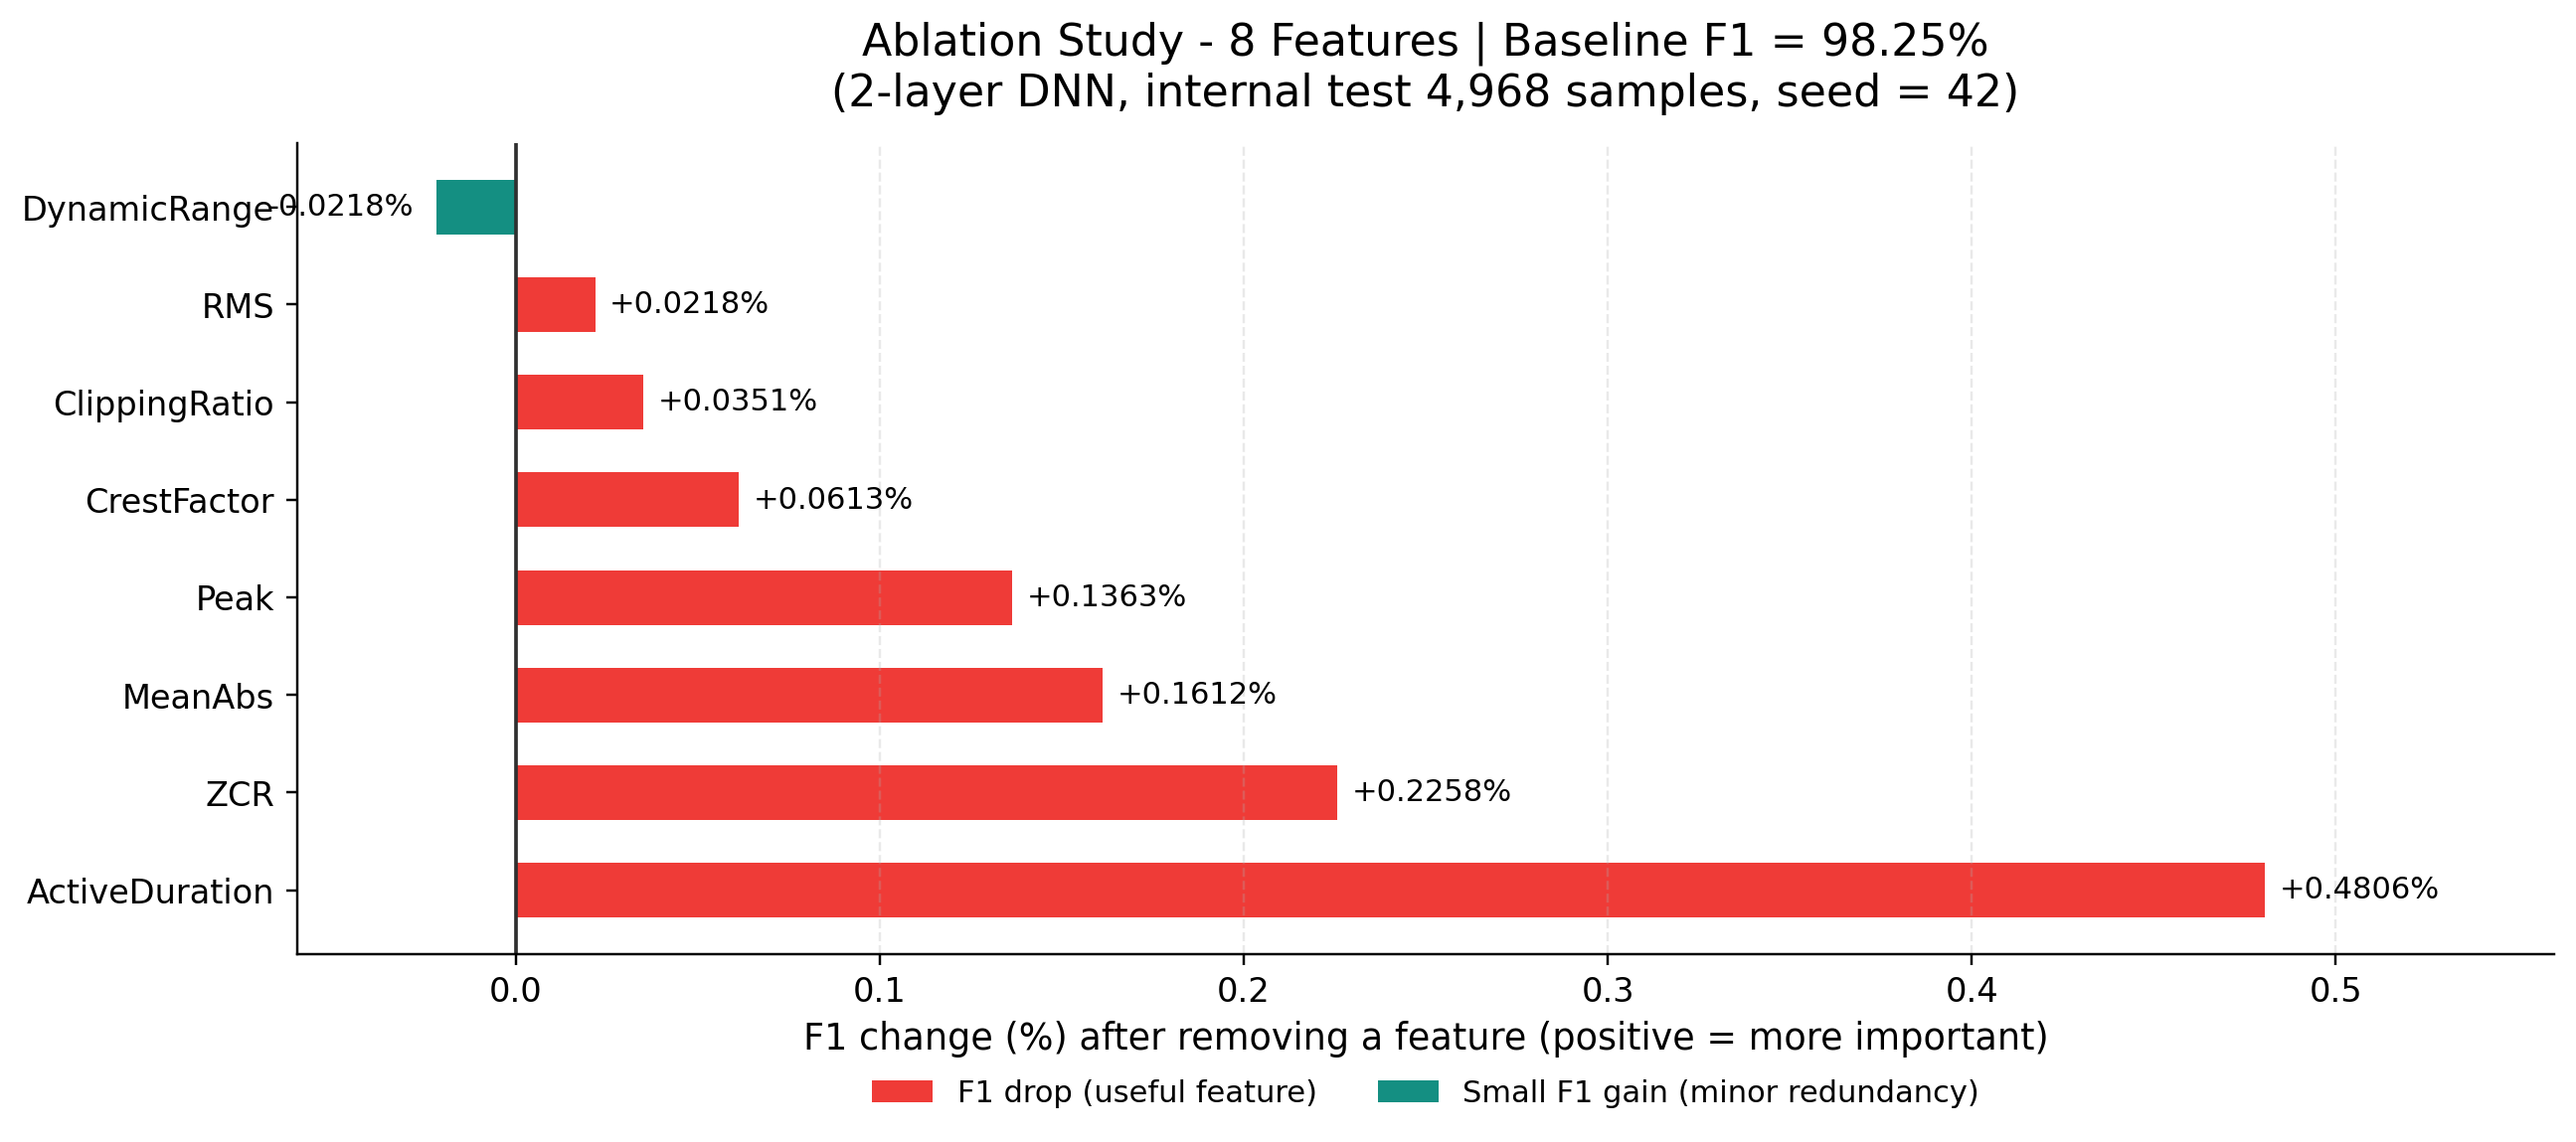
\includegraphics[width=0.92\textwidth]{image1_clean.png}
\caption{Feature ablation summary for the eight handcrafted descriptors. Positive values indicate F1 reduction after a feature is removed, so larger bars correspond to more important cues.}
\label{fig:ablation}
\end{figure}

\subsection{t-SNE Visualization and Domain Shift}

t-SNE was applied to 6{,}668 evaluation samples, consisting of the 4{,}968-sample internal test partition and the 1{,}700-sample external holdout set. The projection used perplexity 40 and seed 42. The analysis was designed to answer two questions: whether bonafide and spoof samples separate in the eight-feature space, and whether internal and external data occupy similar distributions.

The results are shown in Figure~\ref{fig:tsne}. Separation between bonafide and spoof samples is visible, indicating that the feature space carries meaningful anti-spoofing information. At the same time, source-dependent clustering remains clear, exposing the domain mismatch that initially suppressed external performance. In the earlier unadapted setting, external accuracy was only 42.9\%; after 150 external samples per class were added to training, it rose to 84.71\%.

\begin{figure}[htbp]
\centering
\begin{subfigure}[t]{0.48\textwidth}
    \centering
    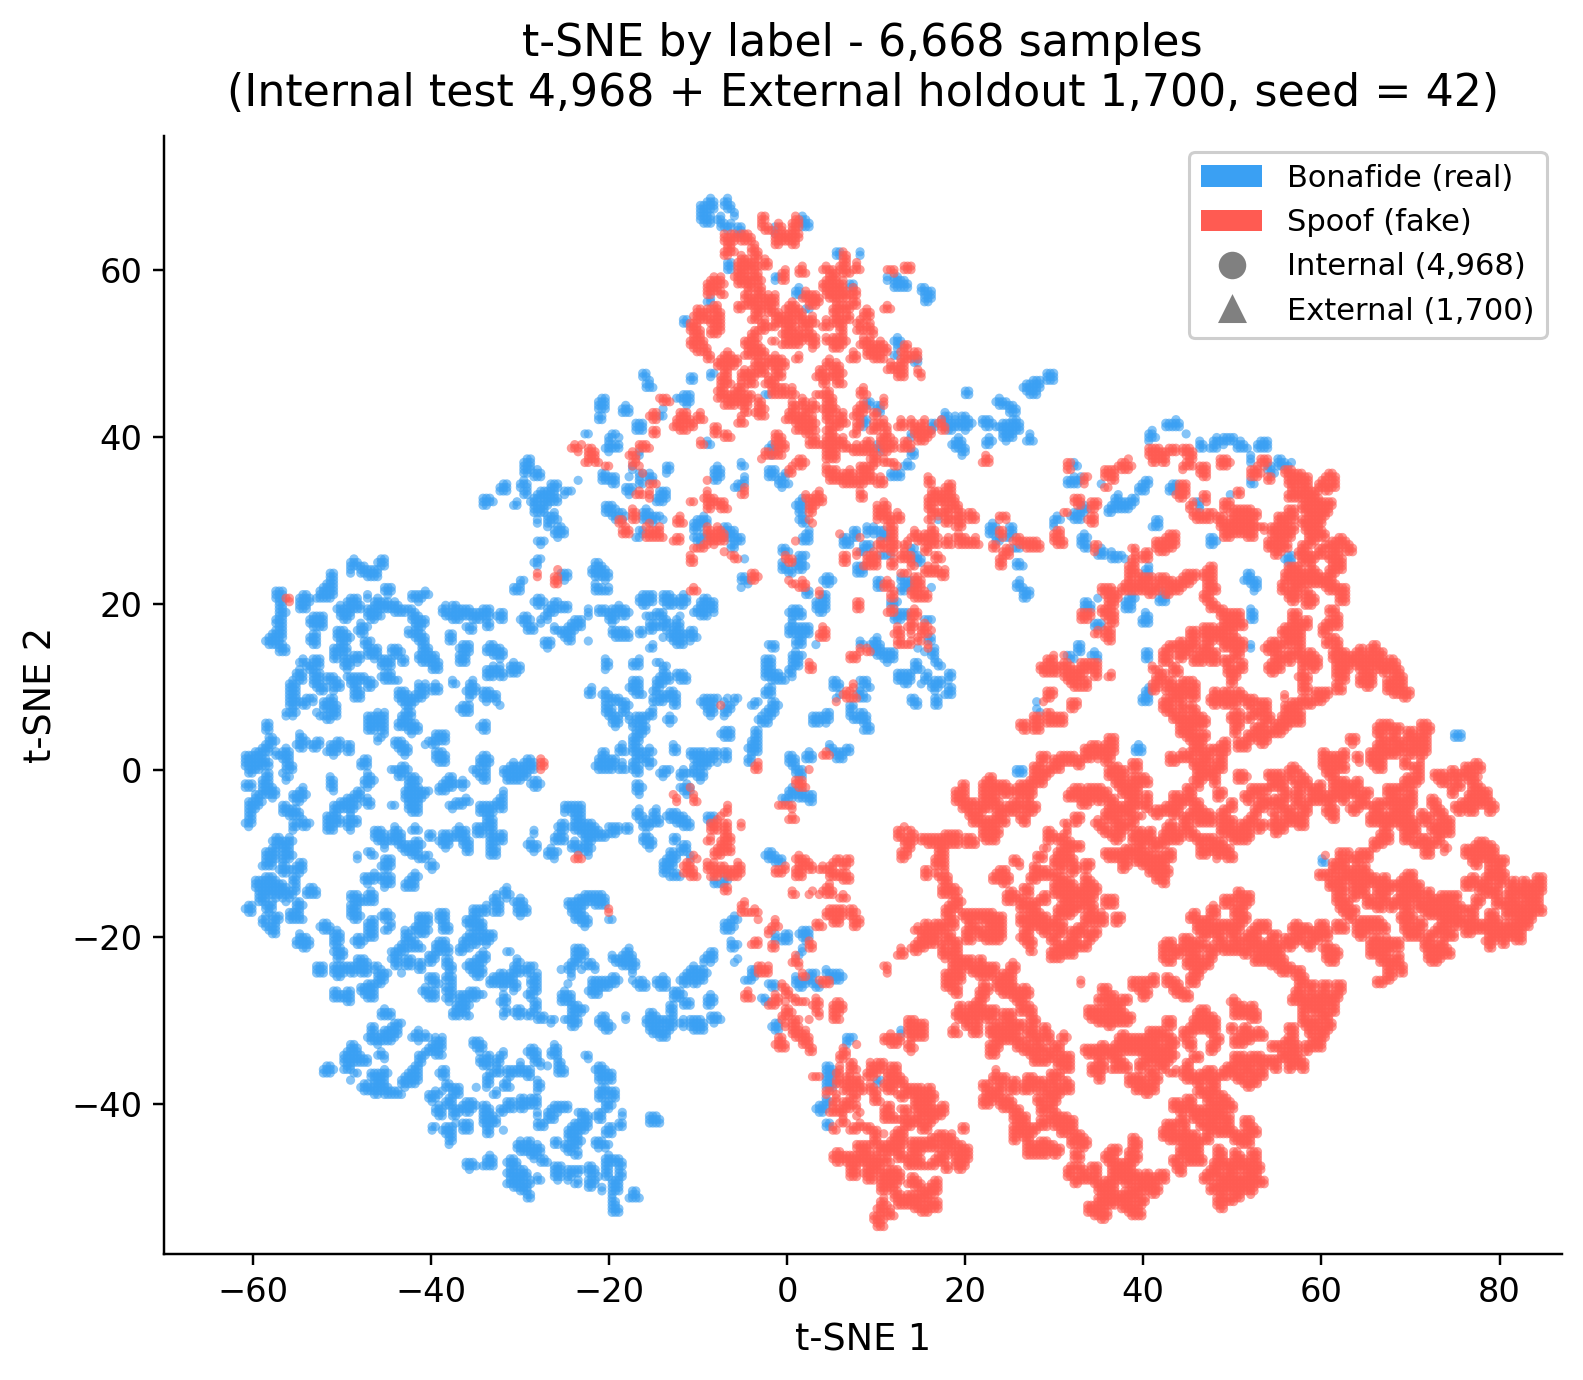
\includegraphics[width=\linewidth]{image11_clean.png}
    \caption{Coloring by label: bonafide vs. spoof.}
\end{subfigure}
\hfill
\begin{subfigure}[t]{0.48\textwidth}
    \centering
    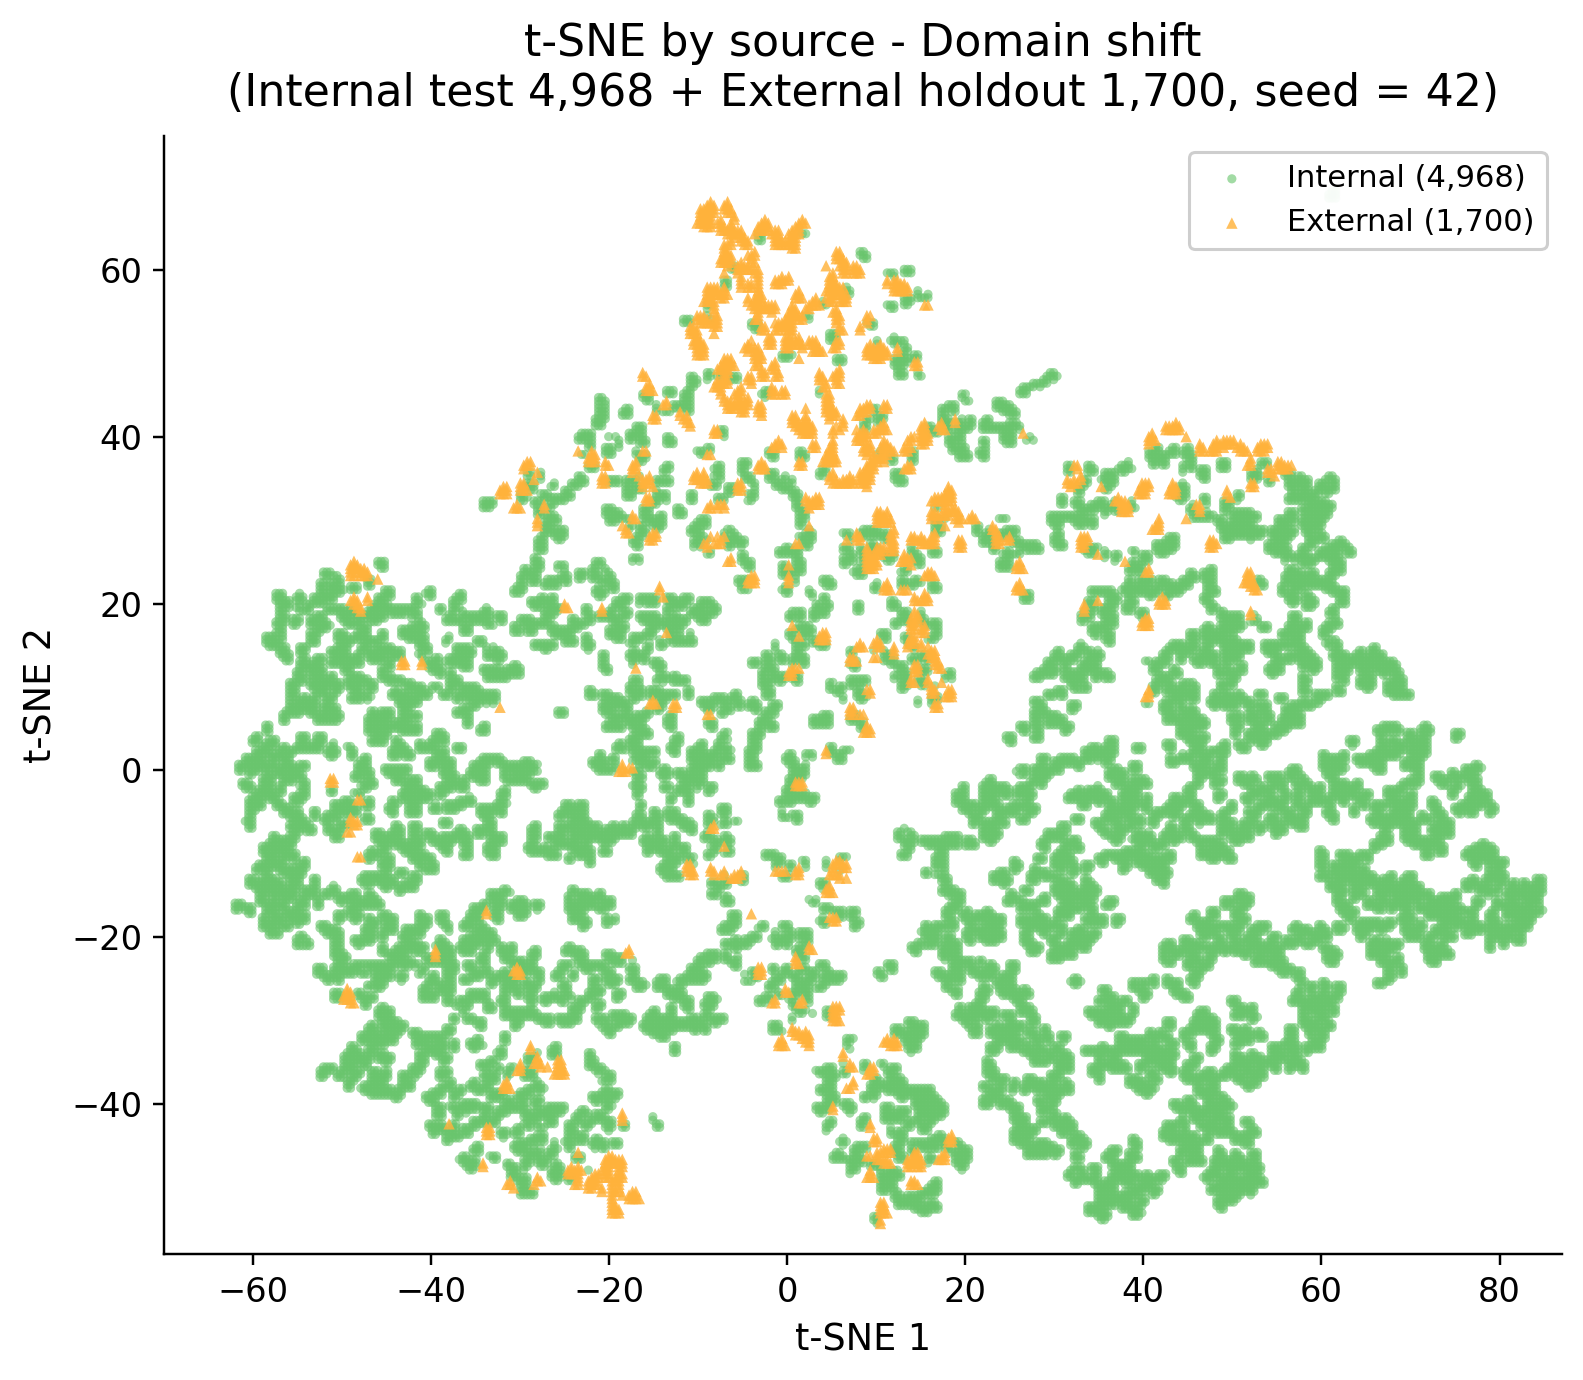
\includegraphics[width=\linewidth]{image12_clean.png}
    \caption{Coloring by source: internal vs. external.}
\end{subfigure}
\caption{t-SNE analysis of the handcrafted feature space. The classes are separable, but a clear source-domain gap remains.}
\label{fig:tsne}
\end{figure}

\subsection{Three-Model Comparison}

The comparative study used the following setup: 24{,}840 internal training samples, an additional 150 external samples per class for selective mixing, and a final external holdout of 1{,}700 samples with 850 bonafide and 850 spoof examples. A unified threshold of 0.25 was applied to all models for a fair deployment-oriented comparison.

Table~\ref{tab:internal} summarizes internal test results, while Table~\ref{tab:external} reports out-of-source performance. The internal scores show that both Cross-Scale Attention Lite and CBAM-ResNet Lite remain strong on familiar data. The external results are more meaningful for deployment: Cross-Scale Attention Lite provides the most security-oriented balance because it retains high spoof recall while staying smaller than CBAM-ResNet Lite.

\begin{table}[htbp]
\caption{Internal evaluation results.}
\label{tab:internal}
\centering
\small
\begin{tabular}{lcccc}
\toprule
\textbf{Model} & \textbf{Params} & \textbf{TFLite size} & \textbf{Accuracy} & \textbf{F1} \\
\midrule
Cross-Scale Attention Lite & 9{,}313 & 42.2 KB & 98.79\% & 98.80\% \\
AASIST Lite & 1{,}057 & 8.6 KB & 96.03\% & 96.14\% \\
CBAM-ResNet Lite & 14{,}145 & 60.7 KB & 98.47\% & 98.49\% \\
\botrule
\end{tabular}
\end{table}

\begin{table}[htbp]
\caption{External holdout results at threshold 0.25.}
\label{tab:external}
\centering
\small
\begin{tabular}{lccccccc}
\toprule
\textbf{Model} & \textbf{Accuracy} & \textbf{Recall} & \textbf{Precision} & \textbf{F1} & \textbf{FAR} & \textbf{FRR} & \textbf{EER} \\
\midrule
Cross-Scale Attention Lite & 85.29\% & 97.65\% & 78.30\% & 86.91\% & 27.06\% & 2.35\% & 18.24\% \\
AASIST Lite & 70.88\% & 55.88\% & 79.83\% & 65.74\% & 14.12\% & 44.12\% & 23.06\% \\
CBAM-ResNet Lite & 85.53\% & 96.47\% & 79.15\% & 86.96\% & 25.41\% & 3.53\% & 18.12\% \\
\botrule
\end{tabular}
\end{table}

The selection of Cross-Scale Attention Lite as the primary Android model is based on deployment trade-offs rather than on one isolated metric. Although CBAM-ResNet Lite remains close numerically on external evaluation, Cross-Scale Attention Lite is about 30\% smaller in TFLite size and uses fewer parameters. AASIST Lite is more compact still, but its spoof recall falls to 55.88\% under the shared threshold, which is too low for a security-focused deployment branch.

\begin{figure}[htbp]
\centering
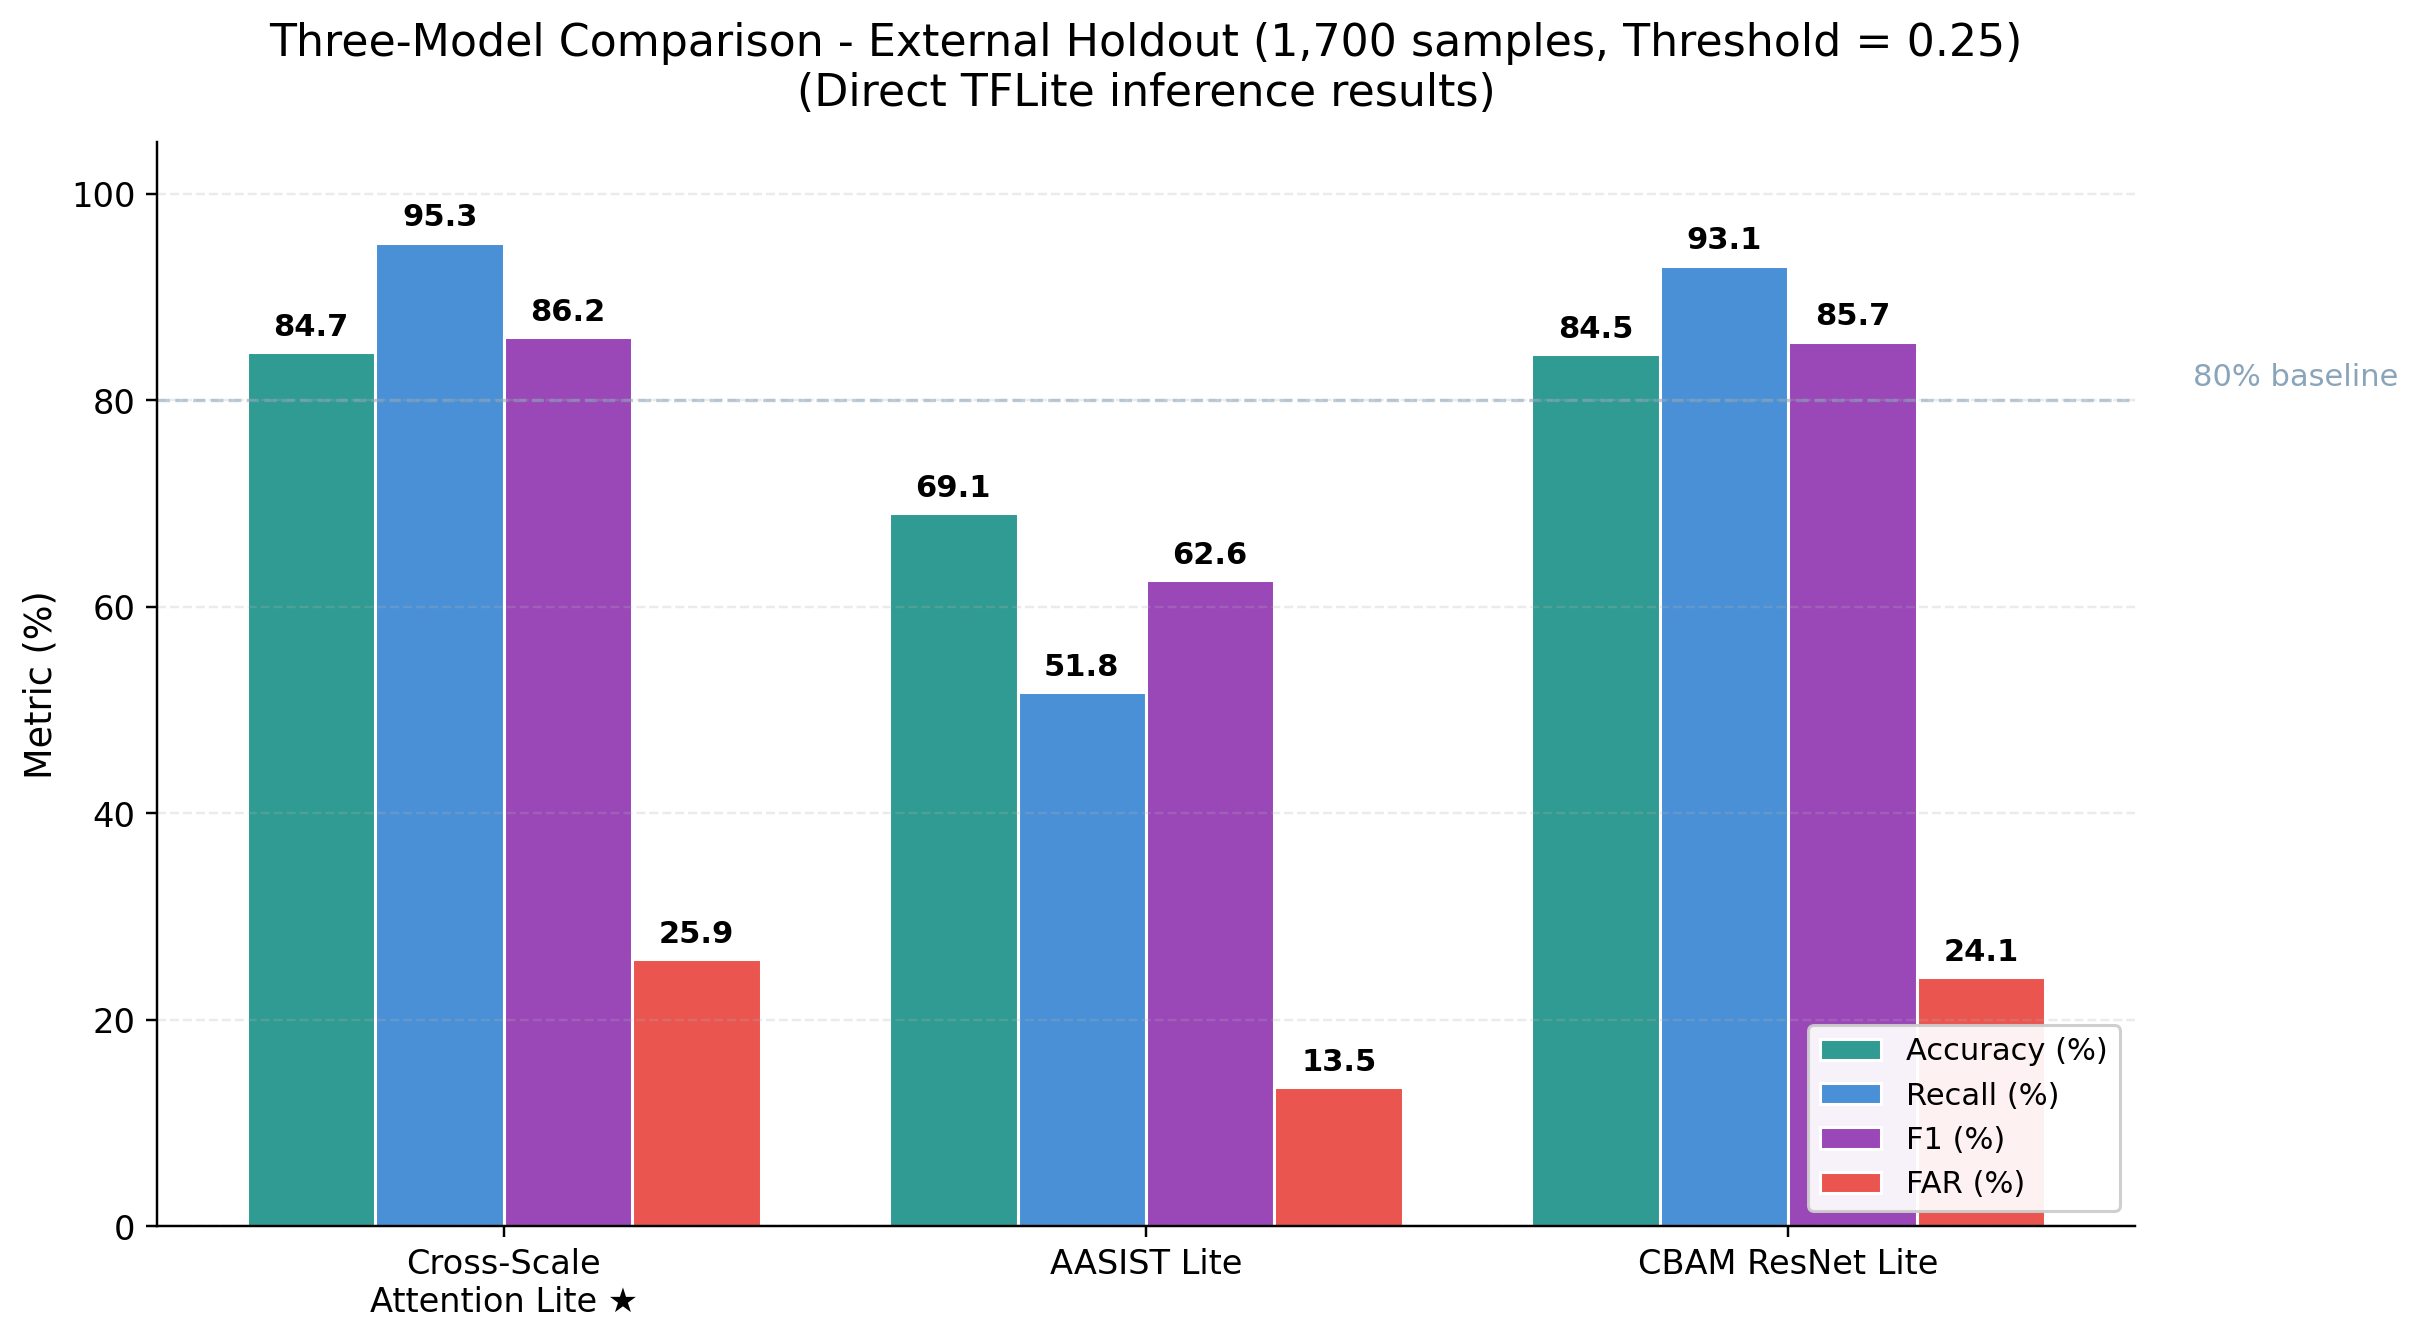
\includegraphics[width=0.86\textwidth]{image10_clean.png}
\caption{External holdout comparison of the three lightweight models from the original project report.}
\label{fig:model-comparison}
\end{figure}

\subsection{Threshold Calibration and Deployment Constraint Check}

The shared threshold of 0.25 is not a casual post-processing choice. It was selected deliberately to emphasize spoof recall, which is more important than user convenience at the current stage of the system. Under this setting, the confusion matrix for Cross-Scale Attention Lite is \textbf{TP = 830, FP = 230, FN = 20, TN = 620}. The corresponding figure is shown in Figure~\ref{fig:confusion}.

\begin{figure}[htbp]
\centering
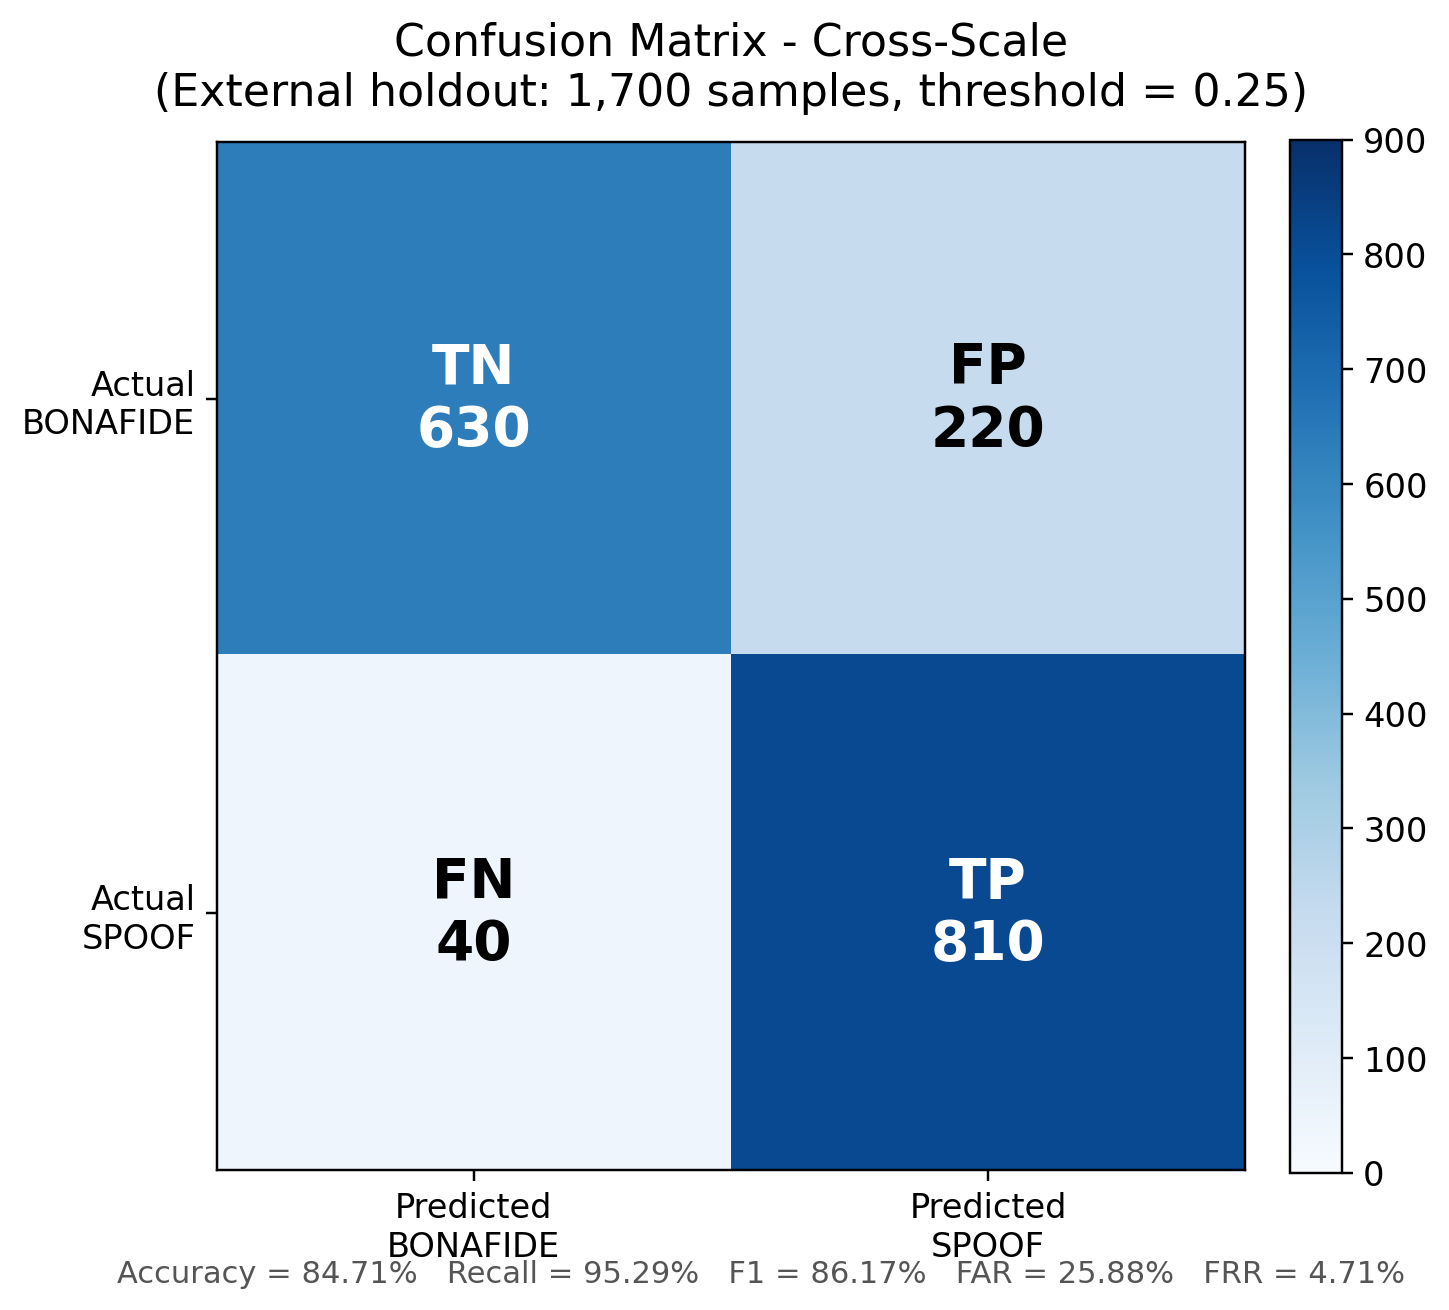
\includegraphics[width=0.52\textwidth]{image9_clean.png}
\caption{Confusion matrix of Cross-Scale Attention Lite on the 1{,}700-sample external holdout at threshold 0.25.}
\label{fig:confusion}
\end{figure}

The deployment branch was also checked against explicit engineering constraints. Table~\ref{tab:acceptance} shows that each target was satisfied.

\begin{table}[htbp]
\caption{Deployment constraint check for the Android branch.}
\label{tab:acceptance}
\centering
\small
\begin{tabular}{lccc}
\toprule
\textbf{Criterion} & \textbf{Target} & \textbf{Achieved} & \textbf{Status} \\
\midrule
External accuracy & $\geq 80\%$ & 85.29\% & Passed \\
Spoof recall & $\geq 85\%$ & 97.65\% & Passed \\
F1-score & $\geq 80\%$ & 86.91\% & Passed \\
TFLite model size & $\leq 100$ KB & 42.2 KB & Passed \\
Pipeline latency & $\leq 500$ ms & 311 ms & Passed \\
RAM usage & $\leq 50$ MB & 14.7 MB & Passed \\
\botrule
\end{tabular}
\end{table}

\section{Android Application Status}\label{sec:android-status}

The application has progressed beyond a proof-of-concept stage and can now function as a credible mobile demonstration artifact. The deployed build supports microphone recording, file-based testing, inference across all three candidate models, threshold-driven decisions, history review, and dataset-related settings. The interface was adjusted so that sample-file analysis now appears in the Detection tab, which is a more natural location for the core workflow.

Figures~\ref{fig:detection} and \ref{fig:sample-tests} now show the current Android user interface used in the latest build.

\begin{figure}[htbp]
\centering
\begin{subfigure}[t]{0.38\textwidth}
    \centering
    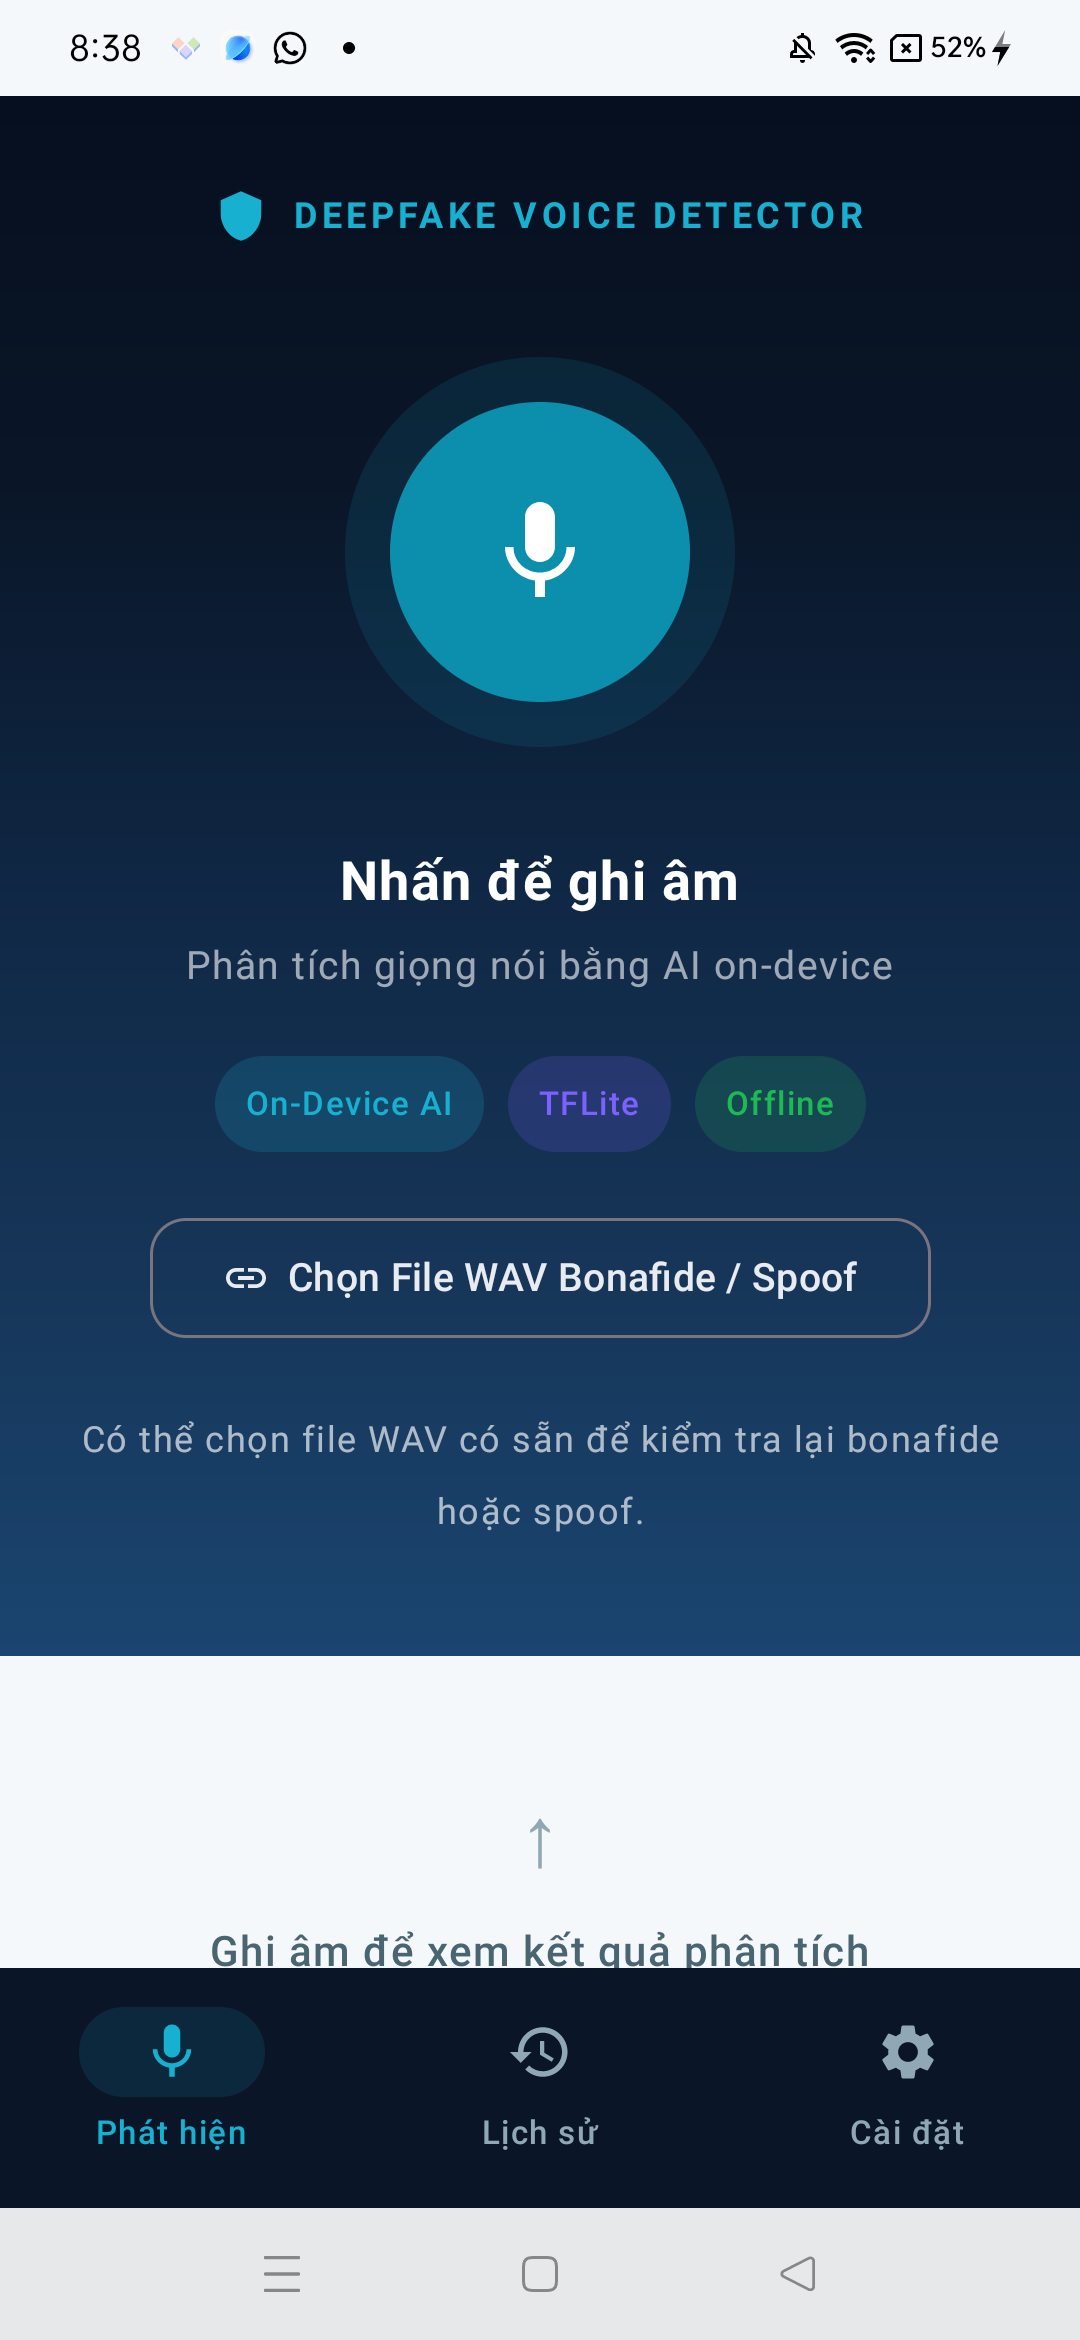
\includegraphics[width=\linewidth]{image3.png}
    \caption{Current Detection tab with microphone control, feature badges, and the integrated WAV file entry point.}
\end{subfigure}
\hfill
\begin{subfigure}[t]{0.38\textwidth}
    \centering
    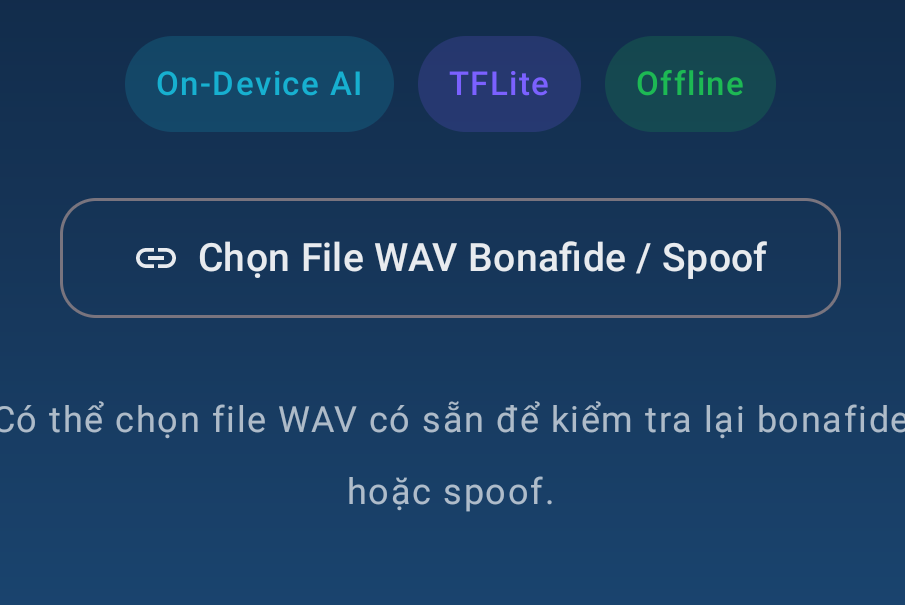
\includegraphics[width=\linewidth]{image4.png}
    \caption{Detail view of the file-selection area now embedded directly inside the Detection workflow.}
\end{subfigure}
\caption{Updated detection workflow after the UI restructuring.}
\label{fig:detection}
\end{figure}

\begin{figure}[htbp]
\centering
\begin{subfigure}[t]{0.38\textwidth}
    \centering
    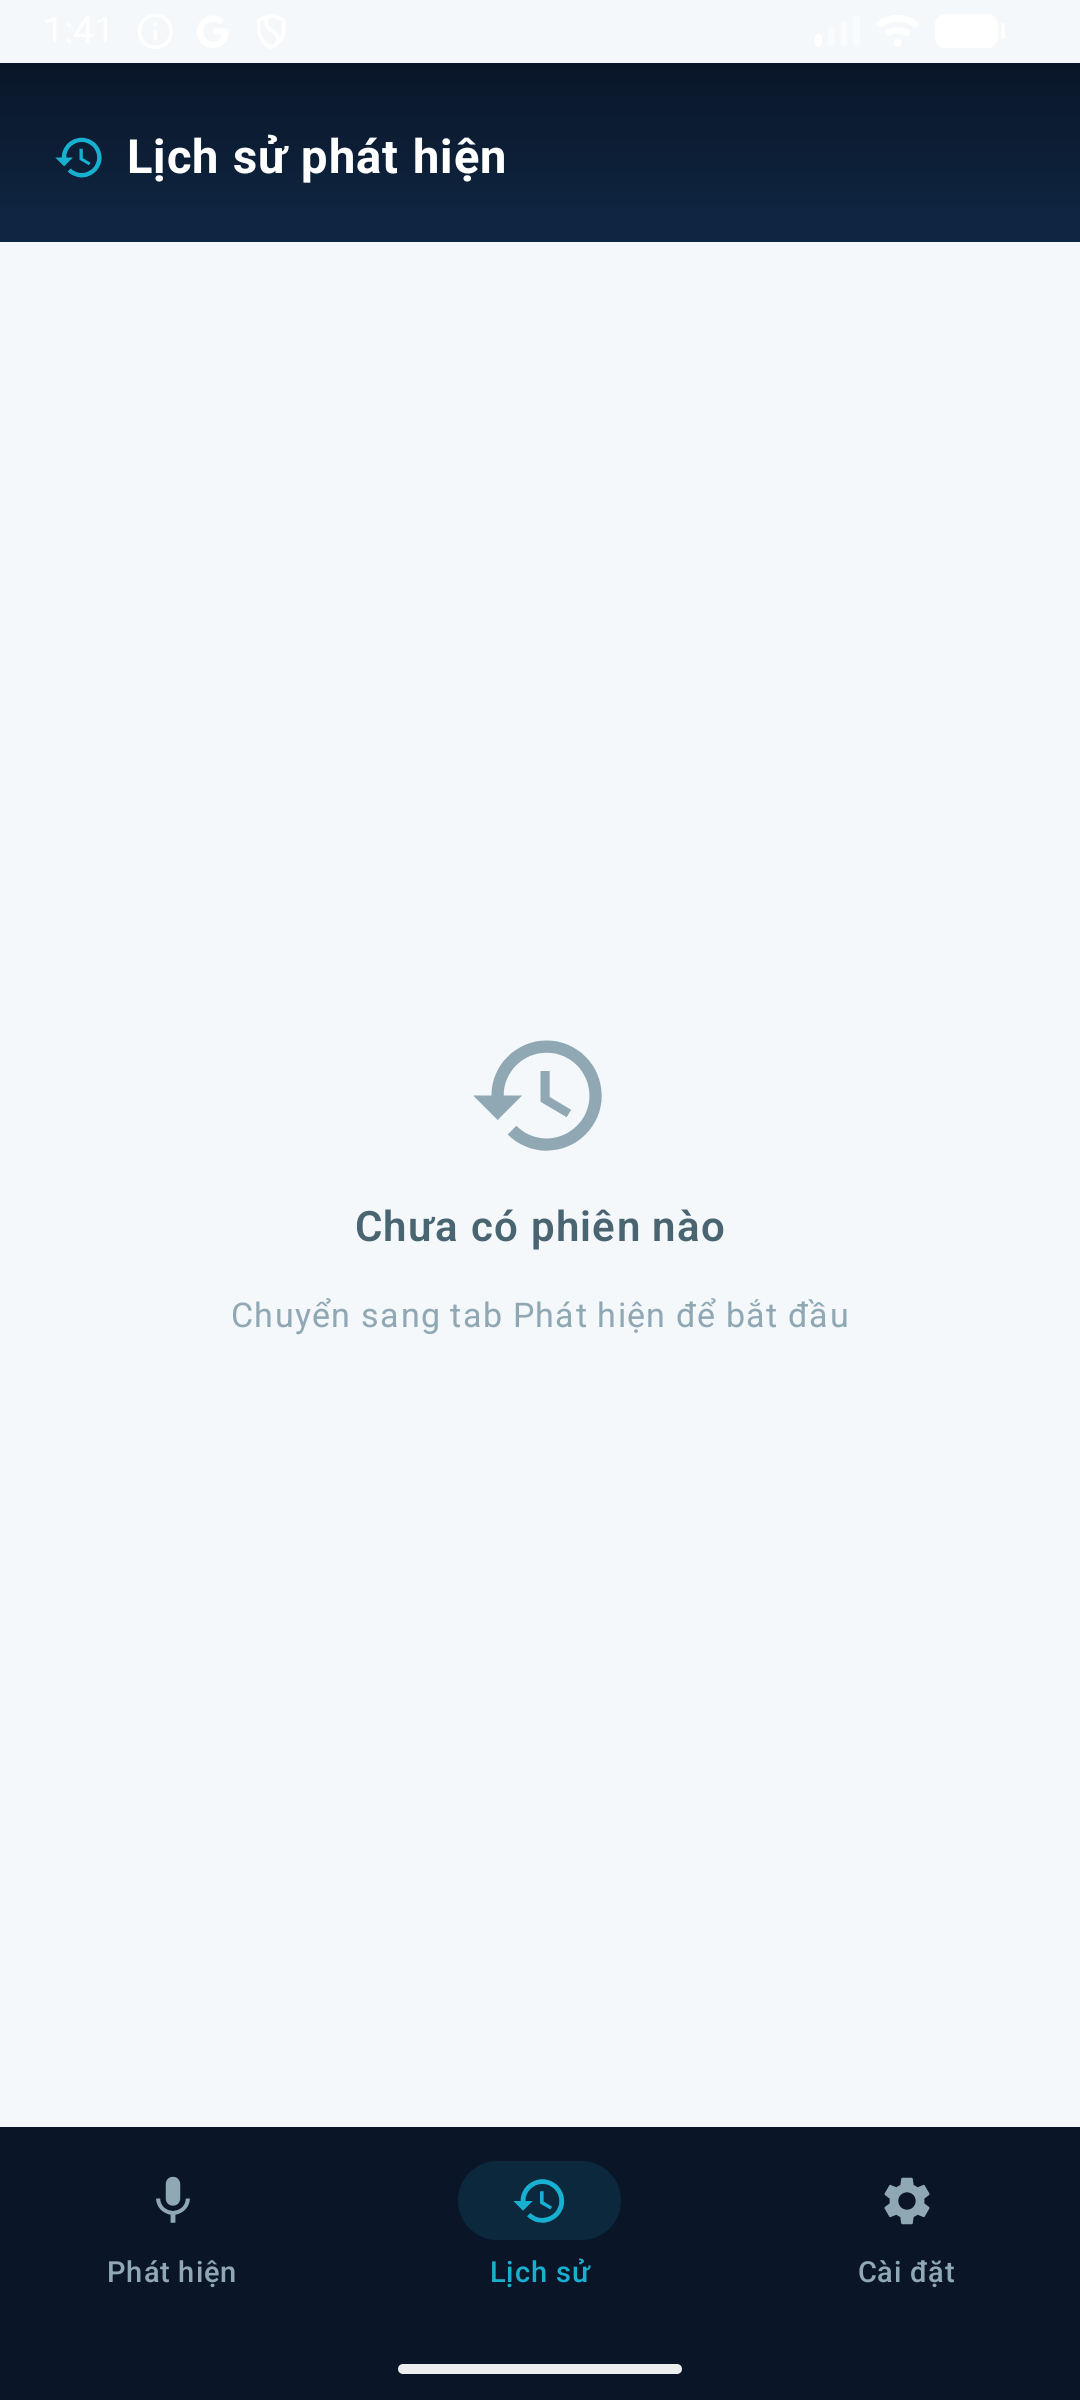
\includegraphics[width=\linewidth]{image5.png}
    \caption{Current History tab before any saved detection session is recorded.}
\end{subfigure}
\hfill
\begin{subfigure}[t]{0.38\textwidth}
    \centering
    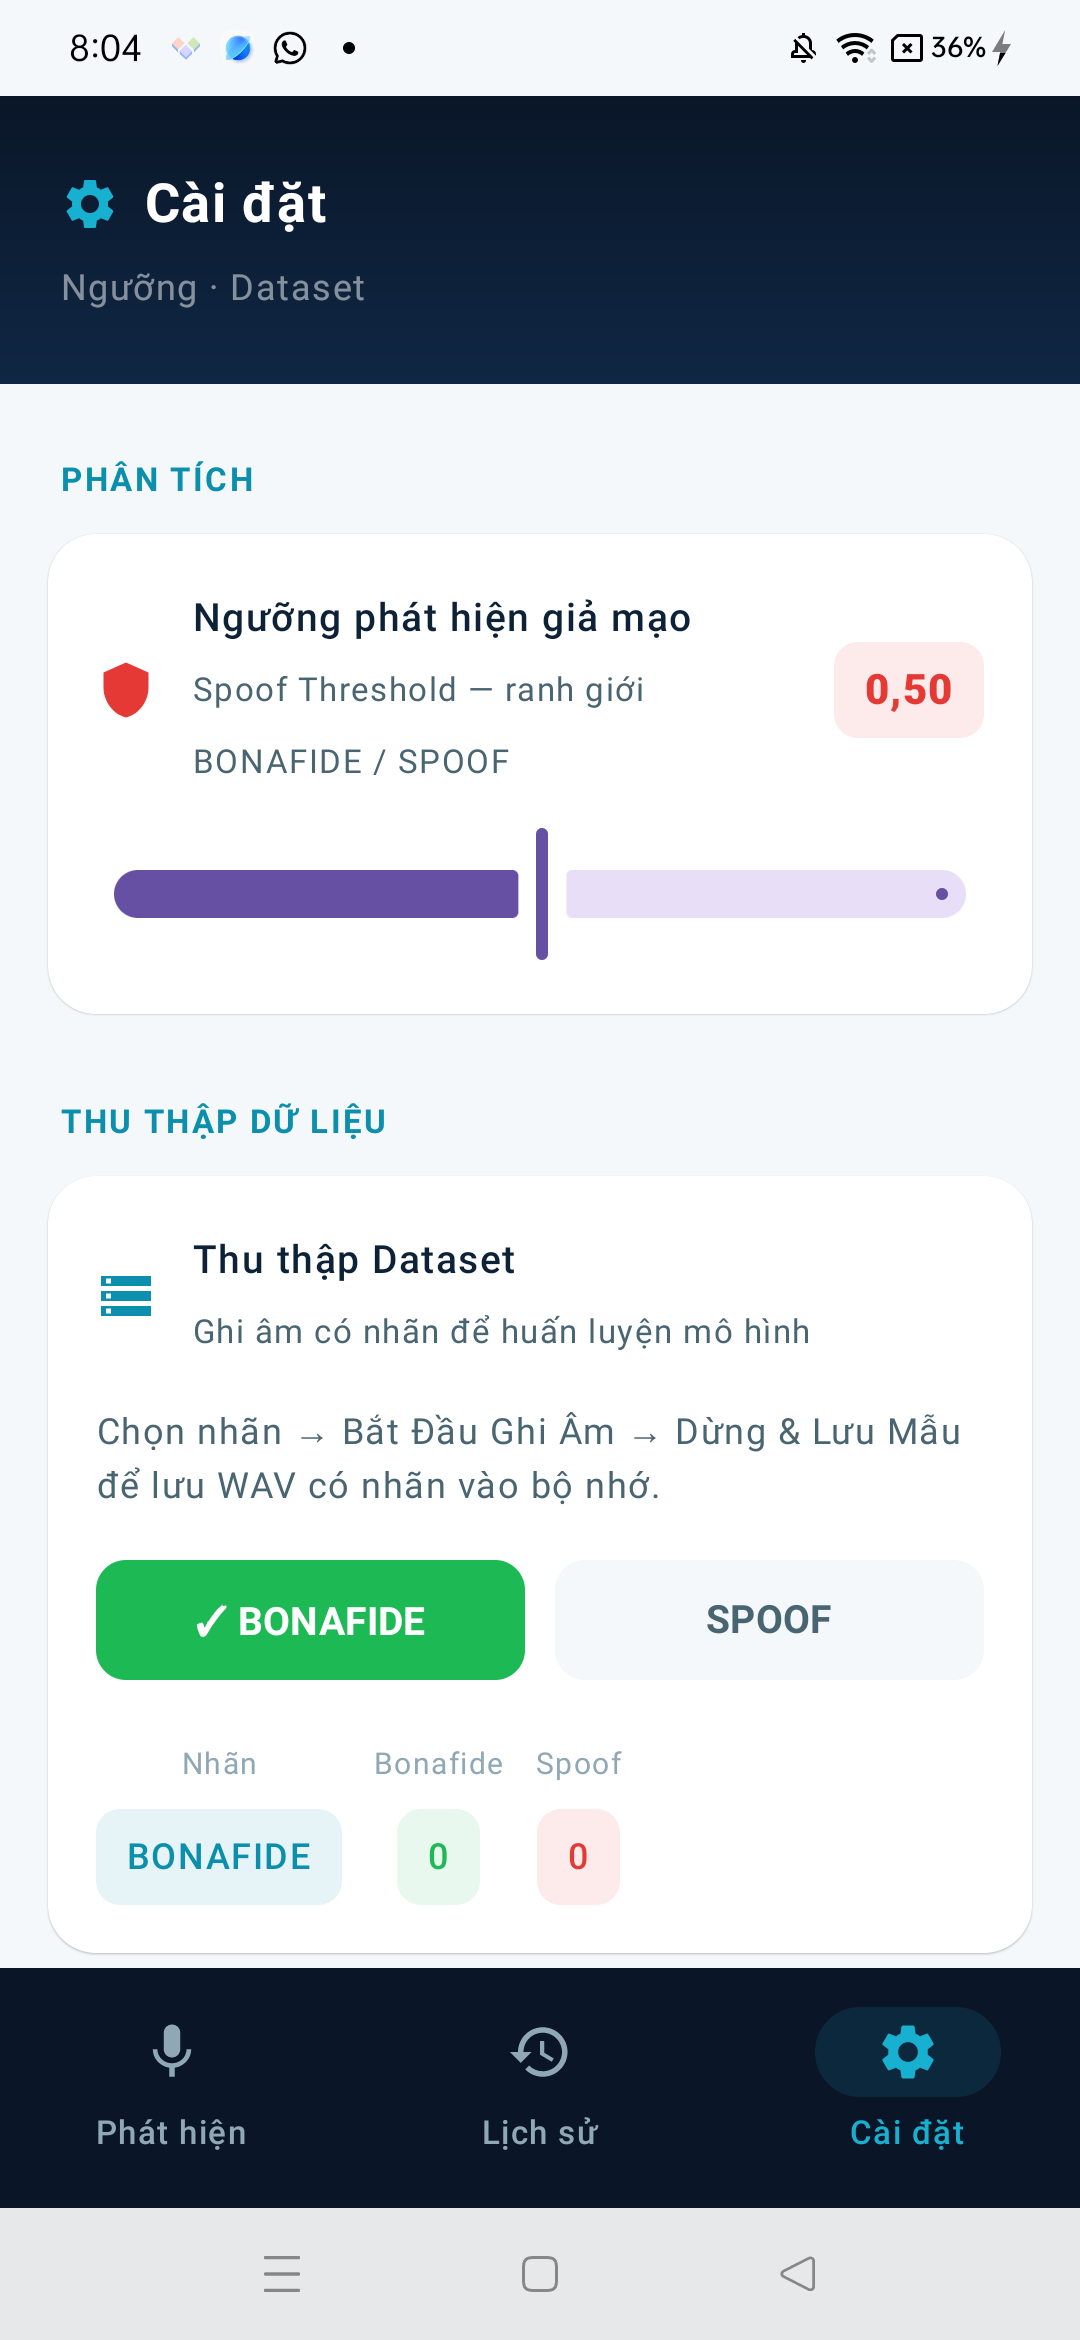
\includegraphics[width=\linewidth]{image6.png}
    \caption{Current Settings tab showing threshold configuration and the dataset collection controls.}
\end{subfigure}
\caption{Additional current application states captured from the updated Android interface.}
\label{fig:sample-tests}
\end{figure}

These screenshots reflect the current user-facing flow more accurately than the earlier report version. In particular, file-based analysis is now initiated directly from the Detection tab through an explicit WAV selection entry point, while the History and Settings tabs remain available as separate surfaces for reviewing stored sessions and managing threshold or dataset-related options.

The supporting \textit{Settings} and \textit{History} screens were also streamlined in this cycle. The settings page now concentrates on threshold, ASV, and dataset configuration, while the history page remains available for reviewing earlier detection sessions.

\section{Discussion}\label{sec:discussion}

The present results support three broader conclusions. First, handcrafted statistical features remain highly competitive when the deployment target is resource-constrained. In this project, their value lies not only in classification quality, but also in predictable runtime cost, implementation simplicity, and ease of explanation during academic review.

Second, the central difficulty in Vietnamese anti-spoofing is not only class separation but also \textit{domain generalization}. The t-SNE analysis indicates that the handcrafted features already distinguish bonafide from spoof samples reasonably well, yet a substantial source shift remains. Mixing 150 external samples per class is effective because it adjusts the boundary inside an already meaningful compact feature space without requiring a heavier domain-adaptation architecture. In practice, this is a lighter alternative to the more elaborate robustness strategies often explored around public anti-spoofing benchmarks \cite{wu2015asvspoof,wang2020asvspoof2019}.

Third, deployment metrics genuinely matter. A larger model may look attractive on benchmark tables and still be a poor Android choice if it complicates packaging, increases latency, or weakens the overall deployment story. Cross-Scale Attention Lite is therefore preferred as the main branch even though CBAM-ResNet Lite remains numerically competitive. The availability of TensorFlow Lite as a mature mobile runtime makes this trade-off practical rather than merely conceptual \cite{tensorflowlite}.

The report also makes the current limitations clear. The false acceptance rate remains fairly high because the threshold was tuned to reduce missed spoof attacks. The external holdout set, while useful, is still modest in scale. In addition, real-device profiling remains necessary so that emulator-based validation can be backed by physical Android measurements.

\section{Limitations and Future Work}\label{sec:plan-requests}

Although the current results are encouraging, several limitations remain. The external holdout set is still relatively small, and broader testing across synthesis engines, microphones, and recording environments would strengthen the generalization claims. The present threshold of 0.25 was selected to prioritize spoof recall, but it also leaves a relatively high false acceptance rate, suggesting that adaptive calibration or cost-aware decision policies deserve further study. In addition, the strongest runtime measurements should ultimately be confirmed on a wider range of physical Android devices rather than relying mainly on emulator-based validation.

\begin{table}[htbp]
\caption{Main directions for future work.}
\label{tab:next-plan}
\centering
\small
\begin{tabular}{p{1.3cm}p{2.6cm}p{6.1cm}p{4.0cm}}
\toprule
\textbf{Track} & \textbf{Scope} & \textbf{Future tasks} & \textbf{Expected outcome} \\
\midrule
Data expansion & External evaluation & Collect more Vietnamese bonafide and spoof samples from diverse synthesis systems, microphones, and acoustic conditions. & Stronger evidence for cross-domain robustness. \\
Runtime validation & Android deployment & Measure latency and RAM usage on a wider set of physical Android devices and chipsets. & More reliable deployment conclusions beyond emulator-based testing. \\
Decision calibration & Inference behavior & Explore threshold adaptation or risk-aware operating points to reduce false acceptance without sharply lowering spoof recall. & Better security--usability trade-off in practical deployment. \\
\botrule
\end{tabular}
\end{table}

Another open question concerns feature design itself. DynamicRange appears weak in internal ablation, so a broader external study is needed to determine whether it truly helps out-of-domain robustness or can be replaced by another low-cost feature. These directions follow naturally from the current results and are consistent with turning the present deployment branch into a more mature publishable system.

\section{Conclusion}\label{sec:conclusion}

This study shows that a carefully engineered lightweight pipeline can support Vietnamese speech anti-spoofing on Android without relying on heavy spectral front ends or large end-to-end models. The final system combines external data expansion, selective domain-mixing retraining, quantitative feature justification, t-SNE-based domain analysis, and successful Android integration of the main TensorFlow Lite model.

The current evidence supports using Cross-Scale Attention Lite as the main Android branch. It satisfies all acceptance targets, reaches 85.29\% external accuracy with 97.65\% spoof recall, and remains substantially smaller than the strongest competing baseline. More importantly, the work establishes a reproducible connection between dataset preparation, benchmark protocol, application runtime, and user-facing demonstration.

Future progress should focus on broader external validation, richer physical-device profiling, and improved operating-point calibration. Even in its current form, however, the proposed system provides a credible baseline for privacy-preserving, on-device Vietnamese anti-spoofing in resource-constrained mobile applications.

\backmatter
\bmhead{Acknowledgments}

The author thanks Dr. Duc-Tho Mai for supervision and continued guidance, and also acknowledges the Academy of Cryptography Techniques for supporting the research and development environment used in this work.

\bibliography{references}

\end{document}
